\documentclass[aspectratio=169,12pt]{beamer}

% Theme and colors
\usetheme{Madrid}
\usecolortheme{whale}
\setbeamertemplate{navigation symbols}{}
\setbeamertemplate{footline}[frame number]

% Packages
\usepackage{amsmath,amssymb,amsthm}
\usepackage{graphicx}
\usepackage{tikz}
\usetikzlibrary{shapes,arrows,positioning,calc,matrix}
\usepackage{booktabs}
\usepackage{array}
\usepackage{multirow}
\usepackage{algorithm}
\usepackage{algorithmic}
\usepackage{xcolor}
\usepackage{hyperref}

% Custom colors
\definecolor{codegreen}{rgb}{0,0.6,0}
\definecolor{codepurple}{rgb}{0.58,0,0.82}
\definecolor{darkblue}{rgb}{0,0,0.7}

% Title information
\title[Arithmetic Coding]{Arithmetic Coding}
\subtitle{Beyond Huffman --- Encoding Messages as Numbers}
\author[Mahesh C]{\textbf{Mahesh C}\\FISAT}
\institute{Federal Institute of Science and Technology (FISAT)\\Multimedia Technology Class}
\date{\today}

\begin{document}

% Title slide
\begin{frame}
    \titlepage
\end{frame}

% Outline
\begin{frame}{Outline}
    \tableofcontents
\end{frame}


%==============================================================================
\section{Motivation: Why Go Beyond Huffman?}
%==============================================================================

\begin{frame}{Huffman's Limitation}
    \begin{columns}
        \begin{column}{0.5\textwidth}
            \textbf{Recall from Huffman:}
            \begin{itemize}
                \item Each symbol gets an integer number of bits
                \item Minimum code length = 1 bit
                \item Optimal among prefix codes
            \end{itemize}
        \end{column}
        \begin{column}{0.5\textwidth}
            \textbf{The Problem:}
            \begin{itemize}
                \item What if a symbol has $p = 0.95$?
                \item Ideal bits: $-\log_2(0.95) = 0.074$ bits
                \item Huffman must use at least 1 bit
                \item That's 13.5x more than needed!
            \end{itemize}
        \end{column}
    \end{columns}
    
    \vspace{0.5cm}
    \begin{block}{Example: Highly Skewed Source}
        \begin{center}
            \begin{tabular}{c|c|c|c}
                \toprule
                Symbol & Probability & Ideal Bits & Huffman Bits \\
                \midrule
                A & 0.95 & 0.074 & 1 \\
                B & 0.05 & 4.322 & 1 \\
                \bottomrule
            \end{tabular}
        \end{center}
        Entropy $H = 0.286$ bits/symbol, but Huffman gives $L_{avg} = 1.0$ bit/symbol.
        
        Efficiency: only 28.6\%!
    \end{block}
\end{frame}

\begin{frame}{The Key Insight}
    \begin{alertblock}{Huffman's Constraint}
        Huffman assigns a \textbf{whole number of bits} to each symbol.
        
        It cannot assign 0.074 bits to a symbol!
    \end{alertblock}
    
    \vspace{0.5cm}
    \begin{block}{Arithmetic Coding's Solution}
        Don't encode symbols one at a time.
        
        Encode the \textbf{entire message} as a single number between 0 and 1!
        
        \vspace{0.2cm}
        This allows \textbf{fractional bits per symbol} --- getting much closer to entropy.
    \end{block}
    
    \vspace{0.3cm}
    \textbf{Think of it this way:}
    \begin{itemize}
        \item Huffman: Each symbol $\rightarrow$ separate codeword
        \item Arithmetic: Entire message $\rightarrow$ one number
    \end{itemize}
\end{frame}


\begin{frame}{A Simple Analogy: The Number Line}
    \begin{center}
        \Large{Imagine a vertical thermometer from 0 to 1}
    \end{center}
    
    \vspace{0.3cm}
    \begin{columns}
        \begin{column}{0.4\textwidth}
            \begin{center}
                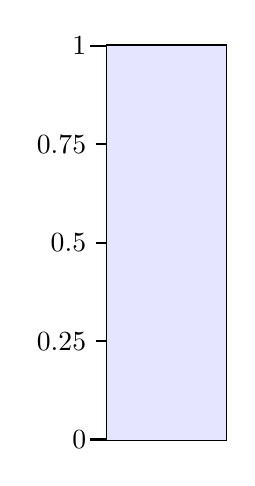
\begin{tikzpicture}[yscale=5, xscale=1.5]
                    % Main bar
                    \draw[very thick] (0,0) rectangle (1,1);
                    \draw[thick] (-0.15,0) -- (0,0) node[left=4pt] {0};
                    \draw[thick] (-0.15,1) -- (0,1) node[left=4pt] {1};
                    \draw[thick] (-0.1,0.5) -- (0,0.5) node[left=4pt] {0.5};
                    \draw[thick] (-0.1,0.25) -- (0,0.25) node[left=4pt] {0.25};
                    \draw[thick] (-0.1,0.75) -- (0,0.75) node[left=4pt] {0.75};
                    
                    % Fill gradient
                    \fill[blue!10] (0,0) rectangle (1,1);
                \end{tikzpicture}
            \end{center}
        \end{column}
        \begin{column}{0.6\textwidth}
            \textbf{The idea:}
            \begin{itemize}
                \item Every possible message maps to a unique sub-interval on this bar
                \item More probable messages get \textbf{taller} intervals
                \item Less probable messages get \textbf{shorter} intervals
                \item Any number inside the interval identifies the message
            \end{itemize}
            
            \vspace{0.3cm}
            \textit{Taller interval = fewer bits to specify = better compression!}
        \end{column}
    \end{columns}
\end{frame}

%==============================================================================
\section{How Arithmetic Coding Works}
%==============================================================================

\begin{frame}{The Basic Idea}
    \begin{block}{Arithmetic Coding in One Sentence}
        Represent the entire message as a \textbf{single floating-point number} in the interval $[0, 1)$ by progressively narrowing a sub-interval based on each symbol's probability.
    \end{block}
    
    \vspace{0.5cm}
    \textbf{Three key concepts:}
    \begin{enumerate}
        \item \textbf{Initial interval:} $[0, 1)$
        \item \textbf{Each symbol narrows the interval} proportionally to its probability
        \item \textbf{Final number:} Any value inside the final interval represents the message
    \end{enumerate}
    
    \vspace{0.3cm}
    \textbf{Notation:}
    \begin{itemize}
        \item $Low$ = lower bound of current interval
        \item $High$ = upper bound of current interval
        \item $Range = High - Low$
    \end{itemize}
\end{frame}


\begin{frame}{Setting Up: Cumulative Probabilities}
    \textbf{Before encoding, assign each symbol a sub-interval of $[0, 1)$:}
    
    \vspace{0.3cm}
    \begin{columns}
        \begin{column}{0.45\textwidth}
            \textbf{Example:} Source $\{A, B, C\}$
            
            \begin{center}
                \begin{tabular}{c|c|c}
                    \toprule
                    Symbol & Prob & Interval \\
                    \midrule
                    A & 0.5 & $[0.0, 0.5)$ \\
                    B & 0.3 & $[0.5, 0.8)$ \\
                    C & 0.2 & $[0.8, 1.0)$ \\
                    \bottomrule
                \end{tabular}
            \end{center}
        \end{column}
        \begin{column}{0.5\textwidth}
            \begin{center}
                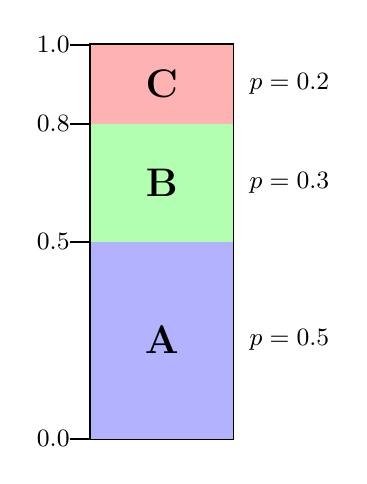
\begin{tikzpicture}[yscale=5, xscale=1.8]
                    % Bar outline
                    \draw[very thick] (0,0) rectangle (1,1);
                    
                    % A region
                    \fill[blue!30] (0,0) rectangle (1,0.5);
                    \node at (0.5,0.25) {\Large\textbf{A}};
                    \node[right] at (1.05,0.25) {\small $p=0.5$};
                    
                    % B region
                    \fill[green!30] (0,0.5) rectangle (1,0.8);
                    \node at (0.5,0.65) {\Large\textbf{B}};
                    \node[right] at (1.05,0.65) {\small $p=0.3$};
                    
                    % C region
                    \fill[red!30] (0,0.8) rectangle (1,1.0);
                    \node at (0.5,0.9) {\Large\textbf{C}};
                    \node[right] at (1.05,0.9) {\small $p=0.2$};
                    
                    % Tick marks
                    \draw[thick] (-0.15,0) -- (0,0) node[left=4pt] {\small 0.0};
                    \draw[thick] (-0.15,0.5) -- (0,0.5) node[left=4pt] {\small 0.5};
                    \draw[thick] (-0.15,0.8) -- (0,0.8) node[left=4pt] {\small 0.8};
                    \draw[thick] (-0.15,1) -- (0,1) node[left=4pt] {\small 1.0};
                \end{tikzpicture}
            \end{center}
        \end{column}
    \end{columns}
\end{frame}

\begin{frame}{The Encoding Algorithm}
    \begin{algorithm}[H]
        \caption{Arithmetic Encoding}
        \begin{algorithmic}[1]
            \STATE \textbf{Input:} Message $m_1 m_2 \ldots m_n$, symbol probabilities
            \STATE \textbf{Output:} A number in $[0, 1)$
            \STATE
            \STATE $Low \leftarrow 0.0$
            \STATE $High \leftarrow 1.0$
            \FOR{each symbol $m_i$ in the message}
                \STATE $Range \leftarrow High - Low$
                \STATE $High \leftarrow Low + Range \times CumulativeHigh(m_i)$
                \STATE $Low \leftarrow Low + Range \times CumulativeLow(m_i)$
            \ENDFOR
            \STATE \textbf{Output} any number in $[Low, High)$
        \end{algorithmic}
    \end{algorithm}
    
    \vspace{0.3cm}
    \textbf{Key formulas:}
    \begin{align*}
        \text{New } High &= Low + Range \times CumulativeHigh(symbol) \\
        \text{New } Low &= Low + Range \times CumulativeLow(symbol)
    \end{align*}
\end{frame}


%==============================================================================
\section{Step-by-Step Example}
%==============================================================================

\begin{frame}{Example: Encode ``BAC''}
    \textbf{Given:} Encode the message \textbf{``BAC''} with:
    
    \begin{columns}
        \begin{column}{0.45\textwidth}
            \begin{center}
                \begin{tabular}{c|c|c}
                    \toprule
                    Symbol & Prob & Interval \\
                    \midrule
                    A & 0.5 & $[0.0, 0.5)$ \\
                    B & 0.3 & $[0.5, 0.8)$ \\
                    C & 0.2 & $[0.8, 1.0)$ \\
                    \bottomrule
                \end{tabular}
            \end{center}
            
            \vspace{0.3cm}
            \textbf{Initial state:}
            \begin{itemize}
                \item $Low = 0.0$
                \item $High = 1.0$
                \item $Range = 1.0$
            \end{itemize}
        \end{column}
        \begin{column}{0.5\textwidth}
            \begin{center}
                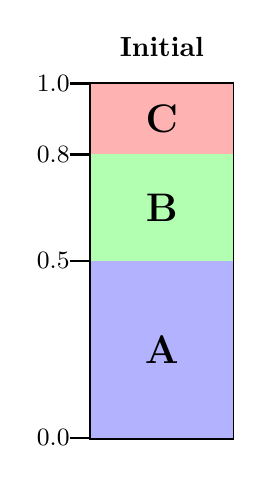
\begin{tikzpicture}[yscale=4.5, xscale=1.8]
                    \draw[very thick] (0,0) rectangle (1,1);
                    \fill[blue!30] (0,0) rectangle (1,0.5);
                    \fill[green!30] (0,0.5) rectangle (1,0.8);
                    \fill[red!30] (0,0.8) rectangle (1,1.0);
                    \node at (0.5,0.25) {\Large\textbf{A}};
                    \node at (0.5,0.65) {\Large\textbf{B}};
                    \node at (0.5,0.9) {\Large\textbf{C}};
                    \draw[thick] (-0.15,0) -- (0,0) node[left=4pt] {\small 0.0};
                    \draw[thick] (-0.15,0.5) -- (0,0.5) node[left=4pt] {\small 0.5};
                    \draw[thick] (-0.15,0.8) -- (0,0.8) node[left=4pt] {\small 0.8};
                    \draw[thick] (-0.15,1) -- (0,1) node[left=4pt] {\small 1.0};
                    \node[above] at (0.5,1.05) {\textbf{Initial}};
                \end{tikzpicture}
            \end{center}
        \end{column}
    \end{columns}
    
    Let's encode symbol by symbol...
\end{frame}


\begin{frame}{Step 1: Encode ``B''}
    \textbf{Current:} $Low = 0.0$, $High = 1.0$, $Range = 1.0$ \quad Symbol B: $[0.5, 0.8)$
    
    \vspace{0.1cm}
    $\text{New } Low = 0.0 + 1.0 \times 0.5 = \mathbf{0.5}$ \qquad $\text{New } High = 0.0 + 1.0 \times 0.8 = \mathbf{0.8}$
    
    \begin{center}
        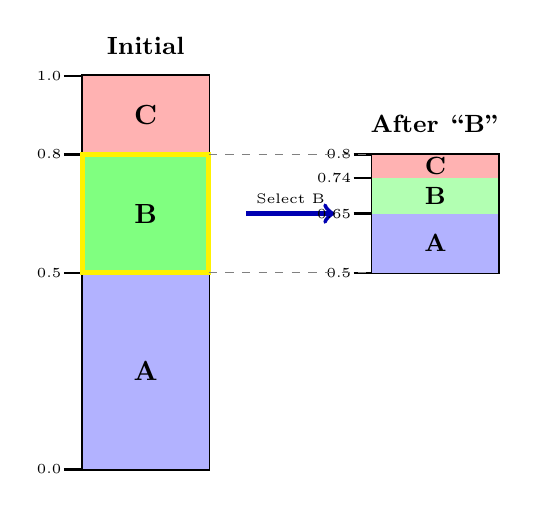
\begin{tikzpicture}[yscale=5, xscale=1.6]
            % --- Bar 1: Initial ---
            \draw[very thick] (0,0) rectangle (1,1);
            \fill[blue!30] (0,0) rectangle (1,0.5);
            \fill[green!50] (0,0.5) rectangle (1,0.8);
            \fill[red!30] (0,0.8) rectangle (1,1.0);
            \node at (0.5,0.25) {\textbf{A}};
            \node at (0.5,0.65) {\textbf{B}};
            \node at (0.5,0.9) {\textbf{C}};
            \draw[thick] (-0.15,0) -- (0,0) node[left=4pt] {\tiny 0.0};
            \draw[thick] (-0.15,0.5) -- (0,0.5) node[left=4pt] {\tiny 0.5};
            \draw[thick] (-0.15,0.8) -- (0,0.8) node[left=4pt] {\tiny 0.8};
            \draw[thick] (-0.15,1) -- (0,1) node[left=4pt] {\tiny 1.0};
            \node[above] at (0.5,1.03) {\small\textbf{Initial}};
            
            % Highlight B
            \draw[yellow, line width=2pt] (0,0.5) rectangle (1,0.8);
            
            % Arrow
            \draw[->,ultra thick, darkblue] (1.3,0.65) -- (2.0,0.65);
            \node[above] at (1.65,0.65) {\tiny Select B};
            
            % --- Bar 2: After B ---
            \begin{scope}[xshift=2.3cm]
                \draw[very thick] (0,0.5) rectangle (1,0.8);
                \fill[blue!30] (0,0.5) rectangle (1,0.65);
                \fill[green!30] (0,0.65) rectangle (1,0.74);
                \fill[red!30] (0,0.74) rectangle (1,0.8);
                \node at (0.5,0.575) {\small\textbf{A}};
                \node at (0.5,0.695) {\small\textbf{B}};
                \node at (0.5,0.77) {\small\textbf{C}};
                \draw[thick] (-0.15,0.5) -- (0,0.5) node[left=4pt] {\tiny 0.5};
                \draw[thick] (-0.15,0.65) -- (0,0.65) node[left=4pt] {\tiny 0.65};
                \draw[thick] (-0.15,0.74) -- (0,0.74) node[left=4pt] {\tiny 0.74};
                \draw[thick] (-0.15,0.8) -- (0,0.8) node[left=4pt] {\tiny 0.8};
                \node[above] at (0.5,0.83) {\small\textbf{After ``B''}};
            \end{scope}
            
            % Dashed context lines
            \draw[dashed, gray] (1,0.5) -- (2.3,0.5);
            \draw[dashed, gray] (1,0.8) -- (2.3,0.8);
        \end{tikzpicture}
    \end{center}
    
    \textbf{After ``B'':} Interval narrowed to $[0.5, 0.8)$, $Range = 0.3$
    
    The new bar is subdivided again into A, B, C proportionally.
\end{frame}


\begin{frame}{Step 2: Encode ``A'' (after ``B'')}
    \textbf{Current:} $Low = 0.5$, $High = 0.8$, $Range = 0.3$ \quad Symbol A: $[0.0, 0.5)$
    
    \vspace{0.1cm}
    $\text{New } Low = 0.5 + 0.3 \times 0.0 = \mathbf{0.5}$ \qquad $\text{New } High = 0.5 + 0.3 \times 0.5 = \mathbf{0.65}$
    
    \begin{center}
        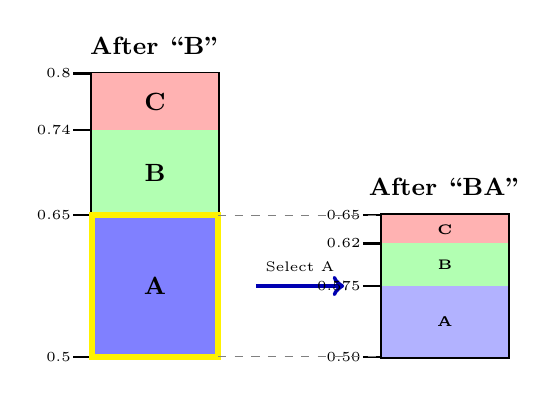
\begin{tikzpicture}[yscale=12, xscale=1.6]
            % --- Bar 1: After B ---
            \draw[very thick] (0,0.5) rectangle (1,0.8);
            \fill[blue!50] (0,0.5) rectangle (1,0.65);
            \fill[green!30] (0,0.65) rectangle (1,0.74);
            \fill[red!30] (0,0.74) rectangle (1,0.8);
            \node at (0.5,0.575) {\small\textbf{A}};
            \node at (0.5,0.695) {\small\textbf{B}};
            \node at (0.5,0.77) {\small\textbf{C}};
            \draw[thick] (-0.15,0.5) -- (0,0.5) node[left=4pt] {\tiny 0.5};
            \draw[thick] (-0.15,0.65) -- (0,0.65) node[left=4pt] {\tiny 0.65};
            \draw[thick] (-0.15,0.74) -- (0,0.74) node[left=4pt] {\tiny 0.74};
            \draw[thick] (-0.15,0.8) -- (0,0.8) node[left=4pt] {\tiny 0.8};
            \node[above] at (0.5,0.81) {\small\textbf{After ``B''}};
            
            % Highlight A
            \draw[yellow, line width=2pt] (0,0.5) rectangle (1,0.65);
            
            % Arrow
            \draw[->,ultra thick, darkblue] (1.3,0.575) -- (2.0,0.575);
            \node[above] at (1.65,0.58) {\tiny Select A};
            
            % --- Bar 2: After BA ---
            \begin{scope}[xshift=2.3cm]
                \draw[very thick] (0,0.5) rectangle (1,0.65);
                \fill[blue!30] (0,0.5) rectangle (1,0.575);
                \fill[green!30] (0,0.575) rectangle (1,0.62);
                \fill[red!30] (0,0.62) rectangle (1,0.65);
                \node at (0.5,0.5375) {\tiny\textbf{A}};
                \node at (0.5,0.5975) {\tiny\textbf{B}};
                \node at (0.5,0.635) {\tiny\textbf{C}};
                \draw[thick] (-0.15,0.5) -- (0,0.5) node[left=4pt] {\tiny 0.50};
                \draw[thick] (-0.15,0.575) -- (0,0.575) node[left=4pt] {\tiny 0.575};
                \draw[thick] (-0.15,0.62) -- (0,0.62) node[left=4pt] {\tiny 0.62};
                \draw[thick] (-0.15,0.65) -- (0,0.65) node[left=4pt] {\tiny 0.65};
                \node[above] at (0.5,0.66) {\small\textbf{After ``BA''}};
            \end{scope}
            
            \draw[dashed, gray] (1,0.5) -- (2.3,0.5);
            \draw[dashed, gray] (1,0.65) -- (2.3,0.65);
        \end{tikzpicture}
    \end{center}
    
    \textbf{After ``BA'':} Interval narrowed to $[0.5, 0.65)$, $Range = 0.15$
\end{frame}


\begin{frame}{Step 3: Encode ``C'' (after ``BA'')}
    \textbf{Current:} $Low = 0.5$, $High = 0.65$, $Range = 0.15$ \quad Symbol C: $[0.8, 1.0)$
    
    \vspace{0.1cm}
    $\text{New } Low = 0.5 + 0.15 \times 0.8 = \mathbf{0.62}$ \qquad $\text{New } High = 0.5 + 0.15 \times 1.0 = \mathbf{0.65}$
    
    \begin{center}
        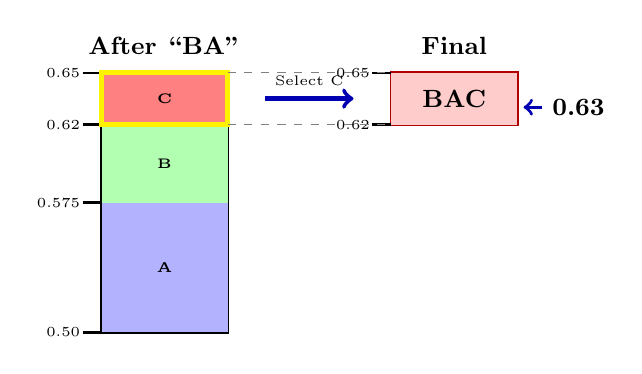
\begin{tikzpicture}[yscale=22, xscale=1.6]
            % --- Bar 1: After BA ---
            \draw[very thick] (0,0.5) rectangle (1,0.65);
            \fill[blue!30] (0,0.5) rectangle (1,0.575);
            \fill[green!30] (0,0.575) rectangle (1,0.62);
            \fill[red!50] (0,0.62) rectangle (1,0.65);
            \node at (0.5,0.5375) {\tiny\textbf{A}};
            \node at (0.5,0.5975) {\tiny\textbf{B}};
            \node at (0.5,0.635) {\tiny\textbf{C}};
            \draw[thick] (-0.15,0.5) -- (0,0.5) node[left=4pt] {\tiny 0.50};
            \draw[thick] (-0.15,0.575) -- (0,0.575) node[left=4pt] {\tiny 0.575};
            \draw[thick] (-0.15,0.62) -- (0,0.62) node[left=4pt] {\tiny 0.62};
            \draw[thick] (-0.15,0.65) -- (0,0.65) node[left=4pt] {\tiny 0.65};
            \node[above] at (0.5,0.655) {\small\textbf{After ``BA''}};
            
            % Highlight C
            \draw[yellow, line width=2pt] (0,0.62) rectangle (1,0.65);
            
            % Arrow
            \draw[->,ultra thick, darkblue] (1.3,0.635) -- (2.0,0.635);
            \node[above] at (1.65,0.637) {\tiny Select C};
            
            % --- Bar 2: After BAC (final) ---
            \begin{scope}[xshift=2.3cm]
                \draw[very thick, red!70!black] (0,0.62) rectangle (1,0.65);
                \fill[red!20] (0,0.62) rectangle (1,0.65);
                \node at (0.5,0.635) {\small\textbf{BAC}};
                \draw[thick] (-0.15,0.62) -- (0,0.62) node[left=4pt] {\tiny 0.62};
                \draw[thick] (-0.15,0.65) -- (0,0.65) node[left=4pt] {\tiny 0.65};
                \node[above] at (0.5,0.655) {\small\textbf{Final}};
                
                % Output marker
                \draw[darkblue, very thick, ->] (1.2,0.63) -- (1.05,0.63);
                \node[right] at (1.2,0.63) {\small\textbf{0.63}};
            \end{scope}
            
            \draw[dashed, gray] (1,0.62) -- (2.3,0.62);
            \draw[dashed, gray] (1,0.65) -- (2.3,0.65);
        \end{tikzpicture}
    \end{center}
    
    \textbf{After ``BAC'':} Final interval $[0.62, 0.65)$. Output: \textbf{0.63}
\end{frame}


\begin{frame}{The Complete Picture: ``BAC'' Encoding}
    \begin{center}
        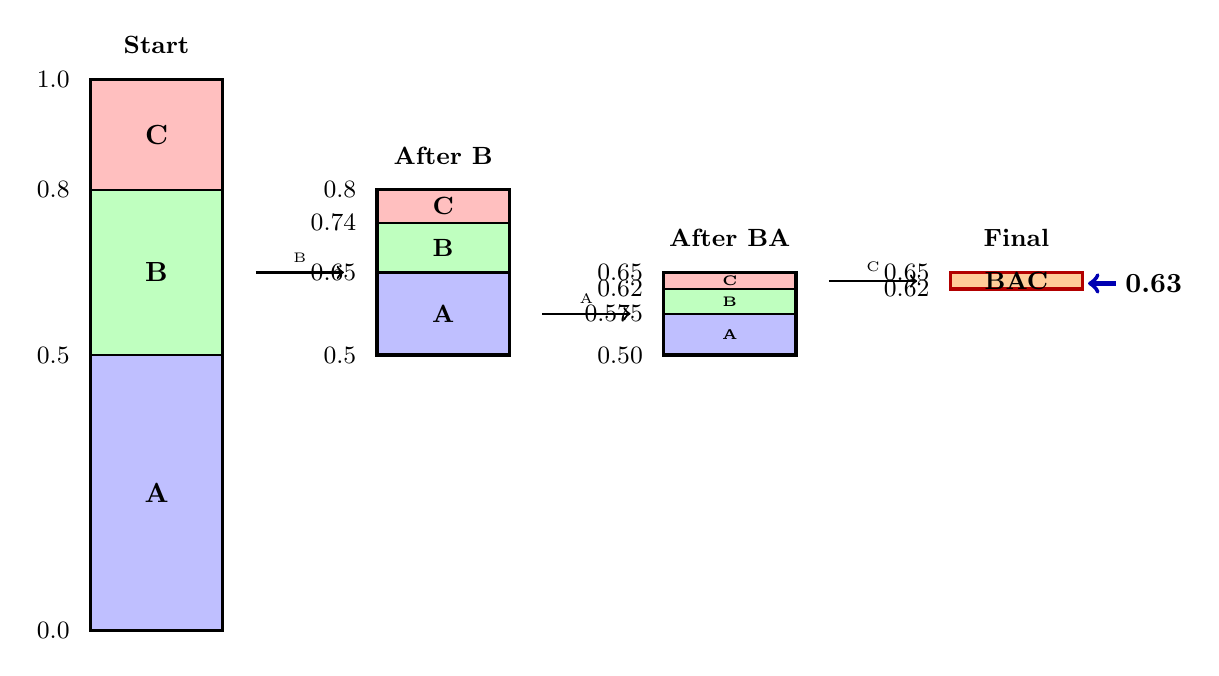
\begin{tikzpicture}[xscale=1.4]
            % --- Bar 1: Initial [0,1) ---
            \fill[blue!25] (0,0) rectangle (1.2,3.5);
            \fill[green!25] (0,3.5) rectangle (1.2,5.6);
            \fill[red!25] (0,5.6) rectangle (1.2,7);
            \draw[very thick] (0,0) rectangle (1.2,7);
            \draw[thick] (0,3.5) -- (1.2,3.5);
            \draw[thick] (0,5.6) -- (1.2,5.6);
            \node at (0.6,1.75) {\textbf{A}};
            \node at (0.6,4.55) {\textbf{B}};
            \node at (0.6,6.3) {\textbf{C}};
            \node[left] at (-0.1,0) {\small 0.0};
            \node[left] at (-0.1,3.5) {\small 0.5};
            \node[left] at (-0.1,5.6) {\small 0.8};
            \node[left] at (-0.1,7) {\small 1.0};
            \node[above] at (0.6,7.2) {\small\textbf{Start}};
            
            % Arrow 1
            \draw[->,thick] (1.5,4.55) -- (2.3,4.55);
            \node[above] at (1.9,4.55) {\tiny B};
            
            % --- Bar 2: After B [0.5, 0.8) ---
            \begin{scope}[xshift=2.6cm]
                \fill[blue!25] (0,3.5) rectangle (1.2,4.55);
                \fill[green!25] (0,4.55) rectangle (1.2,5.18);
                \fill[red!25] (0,5.18) rectangle (1.2,5.6);
                \draw[very thick] (0,3.5) rectangle (1.2,5.6);
                \draw[thick] (0,4.55) -- (1.2,4.55);
                \draw[thick] (0,5.18) -- (1.2,5.18);
                \node at (0.6,4.025) {\small\textbf{A}};
                \node at (0.6,4.865) {\small\textbf{B}};
                \node at (0.6,5.39) {\small\textbf{C}};
                \node[left] at (-0.1,3.5) {\small 0.5};
                \node[left] at (-0.1,4.55) {\small 0.65};
                \node[left] at (-0.1,5.18) {\small 0.74};
                \node[left] at (-0.1,5.6) {\small 0.8};
                \node[above] at (0.6,5.8) {\small\textbf{After B}};
            \end{scope}
            
            % Arrow 2
            \draw[->,thick] (4.1,4.025) -- (4.9,4.025);
            \node[above] at (4.5,4.025) {\tiny A};
            
            % --- Bar 3: After BA [0.5, 0.65) ---
            \begin{scope}[xshift=5.2cm]
                \fill[blue!25] (0,3.5) rectangle (1.2,4.025);
                \fill[green!25] (0,4.025) rectangle (1.2,4.34);
                \fill[red!25] (0,4.34) rectangle (1.2,4.55);
                \draw[very thick] (0,3.5) rectangle (1.2,4.55);
                \draw[thick] (0,4.025) -- (1.2,4.025);
                \draw[thick] (0,4.34) -- (1.2,4.34);
                \node at (0.6,3.76) {\tiny\textbf{A}};
                \node at (0.6,4.18) {\tiny\textbf{B}};
                \node at (0.6,4.44) {\tiny\textbf{C}};
                \node[left] at (-0.1,3.5) {\small 0.50};
                \node[left] at (-0.1,4.025) {\small 0.575};
                \node[left] at (-0.1,4.34) {\small 0.62};
                \node[left] at (-0.1,4.55) {\small 0.65};
                \node[above] at (0.6,4.75) {\small\textbf{After BA}};
            \end{scope}
            
            % Arrow 3
            \draw[->,thick] (6.7,4.44) -- (7.5,4.44);
            \node[above] at (7.1,4.44) {\tiny C};
            
            % --- Bar 4: After BAC [0.62, 0.65) ---
            \begin{scope}[xshift=7.8cm]
                \fill[orange!40] (0,4.34) rectangle (1.2,4.55);
                \draw[very thick, red!70!black] (0,4.34) rectangle (1.2,4.55);
                \node at (0.6,4.445) {\small\textbf{BAC}};
                \node[left] at (-0.1,4.34) {\small 0.62};
                \node[left] at (-0.1,4.55) {\small 0.65};
                \node[above] at (0.6,4.75) {\small\textbf{Final}};
                
                % Output pointer
                \draw[darkblue, ultra thick, ->] (1.5,4.41) -- (1.25,4.41);
                \node[right] at (1.5,4.41) {\textbf{0.63}};
            \end{scope}
        \end{tikzpicture}
    \end{center}
    
    \vspace{0.2cm}
    The interval narrows with each symbol. Any number in $[0.62, 0.65)$ decodes to ``BAC''.
\end{frame}


\begin{frame}{How Many Bits Did We Use?}
    \textbf{Final interval width:} $0.65 - 0.62 = 0.03$
    
    \vspace{0.3cm}
    \textbf{Bits needed:}
    \begin{equation*}
        \text{Bits} = \lceil -\log_2(0.03) \rceil = \lceil 5.06 \rceil = 6 \text{ bits}
    \end{equation*}
    
    \vspace{0.3cm}
    \textbf{Comparison:}
    \begin{center}
        \begin{tabular}{l|c}
            \toprule
            Method & Bits for ``BAC'' \\
            \midrule
            Fixed-length (2 bits each) & 6 bits \\
            Huffman & 5 bits \\
            Arithmetic coding & $\sim$5.06 bits \\
            Entropy lower bound & $-\log_2(0.5 \times 0.3 \times 0.2) = 4.91$ bits \\
            \bottomrule
        \end{tabular}
    \end{center}
    
    \vspace{0.3cm}
    \begin{block}{Key Point}
        Arithmetic coding gets closer to the entropy limit, especially for longer messages!
    \end{block}
\end{frame}

%==============================================================================
\section{Decoding}
%==============================================================================

\begin{frame}{Decoding: Reversing the Process}
    \textbf{Given:} Number $0.63$, symbol probabilities, message length = 3
    
    \begin{columns}
        \begin{column}{0.45\textwidth}
            \begin{center}
                \begin{tabular}{c|c|c}
                    \toprule
                    Symbol & Prob & Interval \\
                    \midrule
                    A & 0.5 & $[0.0, 0.5)$ \\
                    B & 0.3 & $[0.5, 0.8)$ \\
                    C & 0.2 & $[0.8, 1.0)$ \\
                    \bottomrule
                \end{tabular}
            \end{center}
        \end{column}
        \begin{column}{0.5\textwidth}
            \begin{block}{Decoding Algorithm}
                \begin{enumerate}
                    \item Look at the received number
                    \item Find which symbol's region contains it
                    \item Output that symbol
                    \item Narrow the interval (same as encoder)
                    \item Repeat
                \end{enumerate}
            \end{block}
        \end{column}
    \end{columns}
\end{frame}


\begin{frame}{Decoding ``0.63'' --- Visual Walkthrough}
    \begin{center}
        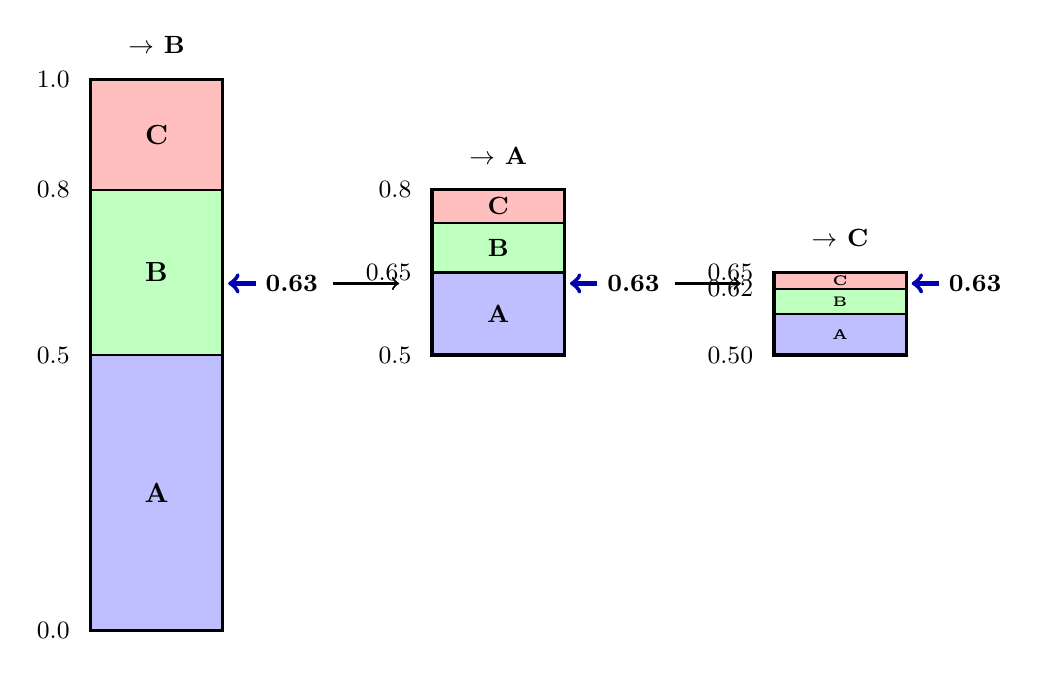
\begin{tikzpicture}[xscale=1.4]
            % --- Bar 1: Where is 0.63? ---
            \fill[blue!25] (0,0) rectangle (1.2,3.5);
            \fill[green!25] (0,3.5) rectangle (1.2,5.6);
            \fill[red!25] (0,5.6) rectangle (1.2,7);
            \draw[very thick] (0,0) rectangle (1.2,7);
            \draw[thick] (0,3.5) -- (1.2,3.5);
            \draw[thick] (0,5.6) -- (1.2,5.6);
            \node at (0.6,1.75) {\textbf{A}};
            \node at (0.6,4.55) {\textbf{B}};
            \node at (0.6,6.3) {\textbf{C}};
            \node[left] at (-0.1,0) {\small 0.0};
            \node[left] at (-0.1,3.5) {\small 0.5};
            \node[left] at (-0.1,5.6) {\small 0.8};
            \node[left] at (-0.1,7) {\small 1.0};
            % Pointer for 0.63
            \draw[darkblue, ultra thick, ->] (1.5,4.41) -- (1.25,4.41);
            \node[right] at (1.5,4.41) {\small\textbf{0.63}};
            \node[above] at (0.6,7.2) {\small\textbf{$\rightarrow$ B}};
            
            % Arrow
            \draw[->,thick] (2.2,4.41) -- (2.8,4.41);
            
            % --- Bar 2: Zoom into B ---
            \begin{scope}[xshift=3.1cm]
                \fill[blue!25] (0,3.5) rectangle (1.2,4.55);
                \fill[green!25] (0,4.55) rectangle (1.2,5.18);
                \fill[red!25] (0,5.18) rectangle (1.2,5.6);
                \draw[very thick] (0,3.5) rectangle (1.2,5.6);
                \draw[thick] (0,4.55) -- (1.2,4.55);
                \draw[thick] (0,5.18) -- (1.2,5.18);
                \node at (0.6,4.025) {\small\textbf{A}};
                \node at (0.6,4.865) {\small\textbf{B}};
                \node at (0.6,5.39) {\small\textbf{C}};
                \node[left] at (-0.1,3.5) {\small 0.5};
                \node[left] at (-0.1,4.55) {\small 0.65};
                \node[left] at (-0.1,5.6) {\small 0.8};
                \draw[darkblue, ultra thick, ->] (1.5,4.41) -- (1.25,4.41);
                \node[right] at (1.5,4.41) {\small\textbf{0.63}};
                \node[above] at (0.6,5.8) {\small\textbf{$\rightarrow$ A}};
            \end{scope}
            
            % Arrow
            \draw[->,thick] (5.3,4.41) -- (5.9,4.41);
            
            % --- Bar 3: Zoom into A ---
            \begin{scope}[xshift=6.2cm]
                \fill[blue!25] (0,3.5) rectangle (1.2,4.025);
                \fill[green!25] (0,4.025) rectangle (1.2,4.34);
                \fill[red!25] (0,4.34) rectangle (1.2,4.55);
                \draw[very thick] (0,3.5) rectangle (1.2,4.55);
                \draw[thick] (0,4.025) -- (1.2,4.025);
                \draw[thick] (0,4.34) -- (1.2,4.34);
                \node at (0.6,3.76) {\tiny\textbf{A}};
                \node at (0.6,4.18) {\tiny\textbf{B}};
                \node at (0.6,4.44) {\tiny\textbf{C}};
                \node[left] at (-0.1,3.5) {\small 0.50};
                \node[left] at (-0.1,4.34) {\small 0.62};
                \node[left] at (-0.1,4.55) {\small 0.65};
                \draw[darkblue, ultra thick, ->] (1.5,4.41) -- (1.25,4.41);
                \node[right] at (1.5,4.41) {\small\textbf{0.63}};
                \node[above] at (0.6,4.75) {\small\textbf{$\rightarrow$ C}};
            \end{scope}
        \end{tikzpicture}
    \end{center}
    
    \vspace{0.2cm}
    \textbf{Decoded:} B $\rightarrow$ A $\rightarrow$ C = \textbf{``BAC''} \checkmark \quad The pointer always lands in the correct region!
\end{frame}

\begin{frame}{Decoding Step by Step (with Math)}
    \textbf{Received number: 0.63}
    
    \vspace{0.3cm}
    \textbf{Step 1:} $Low = 0.0$, $High = 1.0$
    \begin{itemize}
        \item $0.63$ falls in $[0.5, 0.8)$ $\rightarrow$ Symbol = \textbf{B}
        \item Update: $Low = 0.5$, $High = 0.8$
    \end{itemize}
    
    \vspace{0.3cm}
    \textbf{Step 2:} $Low = 0.5$, $High = 0.8$, $Range = 0.3$
    \begin{itemize}
        \item Scaled position: $\frac{0.63 - 0.5}{0.3} = 0.433$
        \item $0.433$ falls in $[0.0, 0.5)$ $\rightarrow$ Symbol = \textbf{A}
        \item Update: $Low = 0.5$, $High = 0.65$
    \end{itemize}
    
    \vspace{0.3cm}
    \textbf{Step 3:} $Low = 0.5$, $High = 0.65$, $Range = 0.15$
    \begin{itemize}
        \item Scaled position: $\frac{0.63 - 0.5}{0.15} = 0.867$
        \item $0.867$ falls in $[0.8, 1.0)$ $\rightarrow$ Symbol = \textbf{C}
    \end{itemize}
    
    \vspace{0.3cm}
    \textbf{Decoded message:} \textbf{BAC} \checkmark
\end{frame}

\begin{frame}{Decoding Algorithm}
    \begin{algorithm}[H]
        \caption{Arithmetic Decoding}
        \begin{algorithmic}[1]
            \STATE \textbf{Input:} Encoded number $V$, probabilities, message length $n$
            \STATE \textbf{Output:} Decoded message
            \STATE $Low \leftarrow 0.0$, $High \leftarrow 1.0$
            \FOR{$i = 1$ to $n$}
                \STATE $Range \leftarrow High - Low$
                \STATE $ScaledValue \leftarrow \frac{V - Low}{Range}$
                \STATE Find symbol $s$ where $CumLow(s) \leq ScaledValue < CumHigh(s)$
                \STATE Output $s$
                \STATE $High \leftarrow Low + Range \times CumHigh(s)$
                \STATE $Low \leftarrow Low + Range \times CumLow(s)$
            \ENDFOR
        \end{algorithmic}
    \end{algorithm}
\end{frame}


%==============================================================================
\section{Detailed Worked Example}
%==============================================================================

\begin{frame}{Complete Example: Encode ``AABA''}
    \textbf{Given:} Source with probabilities:
    
    \begin{columns}
        \begin{column}{0.45\textwidth}
            \begin{center}
                \begin{tabular}{c|c|c}
                    \toprule
                    Symbol & Prob & Interval \\
                    \midrule
                    A & 0.6 & $[0.0, 0.6)$ \\
                    B & 0.3 & $[0.6, 0.9)$ \\
                    C & 0.1 & $[0.9, 1.0)$ \\
                    \bottomrule
                \end{tabular}
            \end{center}
            
            \textbf{Message:} ``AABA''
            
            \textbf{Initial:} $Low = 0.0$, $High = 1.0$
        \end{column}
        \begin{column}{0.5\textwidth}
            \begin{center}
                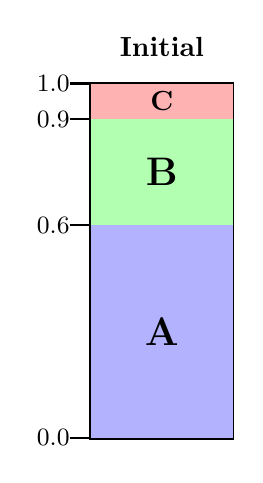
\begin{tikzpicture}[yscale=4.5, xscale=1.8]
                    \draw[very thick] (0,0) rectangle (1,1);
                    \fill[blue!30] (0,0) rectangle (1,0.6);
                    \fill[green!30] (0,0.6) rectangle (1,0.9);
                    \fill[red!30] (0,0.9) rectangle (1,1.0);
                    \node at (0.5,0.3) {\Large\textbf{A}};
                    \node at (0.5,0.75) {\Large\textbf{B}};
                    \node at (0.5,0.95) {\textbf{C}};
                    \draw[thick] (-0.15,0) -- (0,0) node[left=4pt] {\small 0.0};
                    \draw[thick] (-0.15,0.6) -- (0,0.6) node[left=4pt] {\small 0.6};
                    \draw[thick] (-0.15,0.9) -- (0,0.9) node[left=4pt] {\small 0.9};
                    \draw[thick] (-0.15,1) -- (0,1) node[left=4pt] {\small 1.0};
                    \node[above] at (0.5,1.05) {\textbf{Initial}};
                \end{tikzpicture}
            \end{center}
        \end{column}
    \end{columns}
\end{frame}

\begin{frame}{``AABA'' --- Step-by-Step Encoding}
    \textbf{Symbol 1: A} --- $[0.0, 0.6)$
    \begin{align*}
        Low = 0.0 + 1.0 \times 0.0 = 0.0 \qquad High = 0.0 + 1.0 \times 0.6 = 0.6
    \end{align*}
    
    \textbf{Symbol 2: A} --- $Range = 0.6$
    \begin{align*}
        Low = 0.0 + 0.6 \times 0.0 = 0.0 \qquad High = 0.0 + 0.6 \times 0.6 = 0.36
    \end{align*}
    
    \textbf{Symbol 3: B} --- $Range = 0.36$
    \begin{align*}
        Low = 0.0 + 0.36 \times 0.6 = 0.216 \qquad High = 0.0 + 0.36 \times 0.9 = 0.324
    \end{align*}
    
    \textbf{Symbol 4: A} --- $Range = 0.108$
    \begin{align*}
        Low = 0.216 + 0.108 \times 0.0 = 0.216 \qquad High = 0.216 + 0.108 \times 0.6 = 0.2808
    \end{align*}
    
    \textbf{Final interval:} $\boxed{[0.216, 0.2808)}$
\end{frame}


\begin{frame}{``AABA'' --- Complete Vertical Bar Visualization}
    \begin{center}
        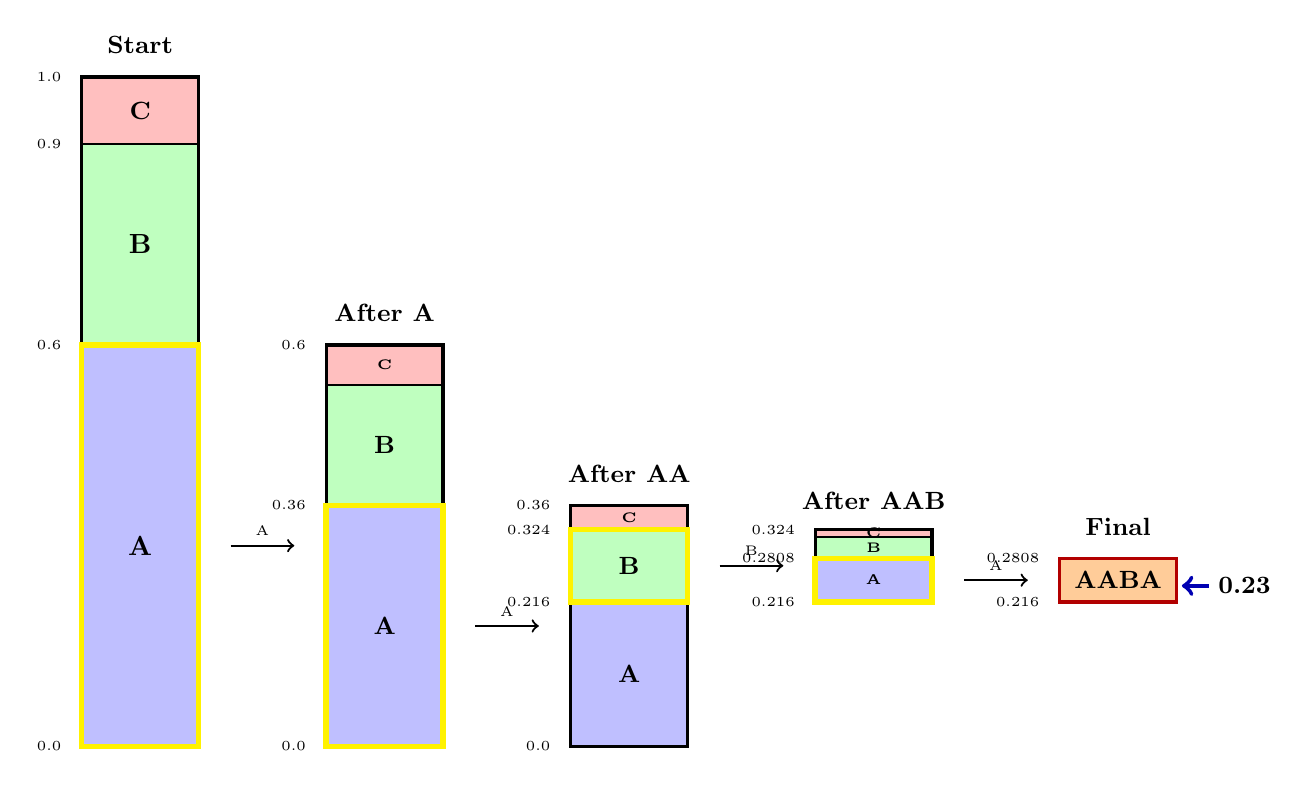
\begin{tikzpicture}[xscale=1.35, yscale=0.85]
            % --- Bar 1: Initial [0,1) ---
            \fill[blue!25] (0,0) rectangle (1.1,6);
            \fill[green!25] (0,6) rectangle (1.1,9);
            \fill[red!25] (0,9) rectangle (1.1,10);
            \draw[very thick] (0,0) rectangle (1.1,10);
            \draw[thick] (0,6) -- (1.1,6);
            \draw[thick] (0,9) -- (1.1,9);
            \node at (0.55,3) {\textbf{A}};
            \node at (0.55,7.5) {\textbf{B}};
            \node at (0.55,9.5) {\small\textbf{C}};
            \node[left] at (-0.1,0) {\tiny 0.0};
            \node[left] at (-0.1,6) {\tiny 0.6};
            \node[left] at (-0.1,9) {\tiny 0.9};
            \node[left] at (-0.1,10) {\tiny 1.0};
            \draw[yellow, line width=2pt] (0,0) rectangle (1.1,6);
            \node[above] at (0.55,10.2) {\small\textbf{Start}};
            
            \draw[->,thick] (1.4,3) -- (2.0,3);
            \node[above] at (1.7,3) {\tiny A};
            
            % --- Bar 2: After A [0, 0.6) ---
            \begin{scope}[xshift=2.3cm]
                \fill[blue!25] (0,0) rectangle (1.1,3.6);
                \fill[green!25] (0,3.6) rectangle (1.1,5.4);
                \fill[red!25] (0,5.4) rectangle (1.1,6);
                \draw[very thick] (0,0) rectangle (1.1,6);
                \draw[thick] (0,3.6) -- (1.1,3.6);
                \draw[thick] (0,5.4) -- (1.1,5.4);
                \node at (0.55,1.8) {\small\textbf{A}};
                \node at (0.55,4.5) {\small\textbf{B}};
                \node at (0.55,5.7) {\tiny\textbf{C}};
                \node[left] at (-0.1,0) {\tiny 0.0};
                \node[left] at (-0.1,3.6) {\tiny 0.36};
                \node[left] at (-0.1,6) {\tiny 0.6};
                \draw[yellow, line width=2pt] (0,0) rectangle (1.1,3.6);
                \node[above] at (0.55,6.2) {\small\textbf{After A}};
            \end{scope}
            
            \draw[->,thick] (3.7,1.8) -- (4.3,1.8);
            \node[above] at (4.0,1.8) {\tiny A};
            
            % --- Bar 3: After AA [0, 0.36) ---
            \begin{scope}[xshift=4.6cm]
                \fill[blue!25] (0,0) rectangle (1.1,2.16);
                \fill[green!25] (0,2.16) rectangle (1.1,3.24);
                \fill[red!25] (0,3.24) rectangle (1.1,3.6);
                \draw[very thick] (0,0) rectangle (1.1,3.6);
                \draw[thick] (0,2.16) -- (1.1,2.16);
                \draw[thick] (0,3.24) -- (1.1,3.24);
                \node at (0.55,1.08) {\small\textbf{A}};
                \node at (0.55,2.7) {\small\textbf{B}};
                \node at (0.55,3.42) {\tiny\textbf{C}};
                \node[left] at (-0.1,0) {\tiny 0.0};
                \node[left] at (-0.1,2.16) {\tiny 0.216};
                \node[left] at (-0.1,3.24) {\tiny 0.324};
                \node[left] at (-0.1,3.6) {\tiny 0.36};
                \draw[yellow, line width=2pt] (0,2.16) rectangle (1.1,3.24);
                \node[above] at (0.55,3.8) {\small\textbf{After AA}};
            \end{scope}
            
            \draw[->,thick] (6.0,2.7) -- (6.6,2.7);
            \node[above] at (6.3,2.7) {\tiny B};
            
            % --- Bar 4: After AAB [0.216, 0.324) ---
            \begin{scope}[xshift=6.9cm]
                \fill[blue!25] (0,2.16) rectangle (1.1,2.808);
                \fill[green!25] (0,2.808) rectangle (1.1,3.132);
                \fill[red!25] (0,3.132) rectangle (1.1,3.24);
                \draw[very thick] (0,2.16) rectangle (1.1,3.24);
                \draw[thick] (0,2.808) -- (1.1,2.808);
                \draw[thick] (0,3.132) -- (1.1,3.132);
                \node at (0.55,2.484) {\tiny\textbf{A}};
                \node at (0.55,2.97) {\tiny\textbf{B}};
                \node at (0.55,3.186) {\tiny\textbf{C}};
                \node[left] at (-0.1,2.16) {\tiny 0.216};
                \node[left] at (-0.1,2.808) {\tiny 0.2808};
                \node[left] at (-0.1,3.24) {\tiny 0.324};
                \draw[yellow, line width=2pt] (0,2.16) rectangle (1.1,2.808);
                \node[above] at (0.55,3.4) {\small\textbf{After AAB}};
            \end{scope}
            
            \draw[->,thick] (8.3,2.484) -- (8.9,2.484);
            \node[above] at (8.6,2.484) {\tiny A};
            
            % --- Bar 5: Final AABA [0.216, 0.2808) ---
            \begin{scope}[xshift=9.2cm]
                \fill[orange!40] (0,2.16) rectangle (1.1,2.808);
                \draw[very thick, red!70!black] (0,2.16) rectangle (1.1,2.808);
                \node at (0.55,2.484) {\small\textbf{AABA}};
                \node[left] at (-0.1,2.16) {\tiny 0.216};
                \node[left] at (-0.1,2.808) {\tiny 0.2808};
                \node[above] at (0.55,3.0) {\small\textbf{Final}};
                
                \draw[darkblue, ultra thick, ->] (1.4,2.4) -- (1.15,2.4);
                \node[right] at (1.4,2.4) {\small\textbf{0.23}};
            \end{scope}
        \end{tikzpicture}
    \end{center}
\end{frame}


\begin{frame}{``AABA'' --- Performance Analysis}
    \textbf{Final interval width:} $0.2808 - 0.216 = 0.0648$
    
    \vspace{0.3cm}
    \textbf{Bits needed:}
    \begin{equation*}
        \text{Bits} = \lceil -\log_2(0.0648) \rceil = \lceil 3.948 \rceil = 4 \text{ bits}
    \end{equation*}
    
    \textbf{Entropy of the message:}
    \begin{align*}
        H(\text{``AABA''}) &= -\log_2(P(\text{A})^3 \times P(\text{B})^1) \\
        &= -\log_2(0.6^3 \times 0.3) \\
        &= -\log_2(0.0648) = 3.948 \text{ bits}
    \end{align*}
    
    \begin{alertblock}{Almost Perfect!}
        Arithmetic coding uses $\approx 4$ bits for a message whose entropy is $3.948$ bits.
        
        That's \textbf{99.9\% efficient}!
    \end{alertblock}
\end{frame}

%==============================================================================
\section{Why Arithmetic Coding is Better}
%==============================================================================

\begin{frame}{Arithmetic vs Huffman: The Comparison}
    \begin{center}
        \begin{tabular}{l|c|c}
            \toprule
            \textbf{Property} & \textbf{Huffman} & \textbf{Arithmetic} \\
            \midrule
            Bits per symbol & Integer only & Fractional \\
            Optimality & Among prefix codes & Among all codes \\
            Skewed distributions & Poor & Excellent \\
            Complexity & Simple & More complex \\
            Speed & Fast & Slower \\
            Patent issues & None & Historically yes \\
            \bottomrule
        \end{tabular}
    \end{center}
    
    \vspace{0.5cm}
    \begin{block}{When Does Arithmetic Coding Shine?}
        \begin{itemize}
            \item When one symbol has very high probability ($p > 0.5$)
            \item When the alphabet is small (e.g., binary)
            \item When you need compression very close to entropy
        \end{itemize}
    \end{block}
\end{frame}

\begin{frame}{Concrete Comparison: Binary Source}
    \textbf{Source:} $P(0) = 0.95$, $P(1) = 0.05$
    
    \vspace{0.3cm}
    \textbf{Entropy:} $H = -0.95\log_2(0.95) - 0.05\log_2(0.05) = 0.286$ bits/symbol
    
    \vspace{0.3cm}
    \begin{columns}
        \begin{column}{0.55\textwidth}
            \begin{center}
                \begin{tabular}{l|c|c}
                    \toprule
                    \textbf{Method} & \textbf{Bits/Sym} & \textbf{Efficiency} \\
                    \midrule
                    Fixed-length & 1.000 & 28.6\% \\
                    Huffman & 1.000 & 28.6\% \\
                    Arithmetic & $\approx 0.29$ & $\approx 98.6\%$ \\
                    Entropy & 0.286 & 100\% \\
                    \bottomrule
                \end{tabular}
            \end{center}
        \end{column}
        \begin{column}{0.4\textwidth}
            \begin{center}
                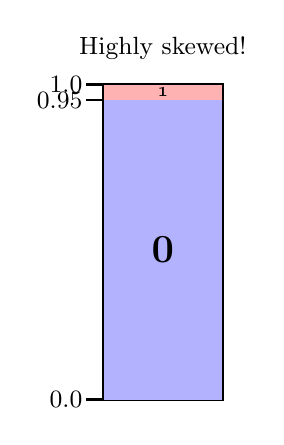
\begin{tikzpicture}[yscale=4, xscale=1.5]
                    \draw[very thick] (0,0) rectangle (1,1);
                    \fill[blue!30] (0,0) rectangle (1,0.95);
                    \fill[red!30] (0,0.95) rectangle (1,1.0);
                    \node at (0.5,0.475) {\Large\textbf{0}};
                    \node at (0.5,0.975) {\tiny\textbf{1}};
                    \draw[thick] (-0.15,0) -- (0,0) node[left=4pt] {\small 0.0};
                    \draw[thick] (-0.15,0.95) -- (0,0.95) node[left=4pt] {\small 0.95};
                    \draw[thick] (-0.15,1) -- (0,1) node[left=4pt] {\small 1.0};
                    \node[above] at (0.5,1.05) {\small Highly skewed!};
                \end{tikzpicture}
            \end{center}
        \end{column}
    \end{columns}
    
    \vspace{0.3cm}
    \begin{alertblock}{Dramatic Difference!}
        For a 1 MB file: Huffman = 1 MB, Arithmetic $\approx$ 290 KB.
    \end{alertblock}
\end{frame}

%==============================================================================
\section{Practical Considerations}
%==============================================================================

\begin{frame}{Problem: Finite Precision}
    \begin{alertblock}{The Biggest Challenge}
        As we encode more symbols, the interval gets \textbf{extremely narrow}.
        
        Computers can't store numbers with infinite precision!
    \end{alertblock}
    
    \vspace{0.3cm}
    \textbf{Example:} After encoding 100 symbols, the interval might be:
    \begin{equation*}
        [0.3749281746291847..., \; 0.3749281746291849...)
    \end{equation*}
    
    This needs more than 64-bit floating point precision!
    
    \vspace{0.3cm}
    \begin{block}{Solution: Incremental Output}
        \begin{itemize}
            \item When both $Low$ and $High$ start with the same leading bits, output those bits immediately
            \item Rescale the interval to use the full $[0, 1)$ range again
            \item This keeps numbers manageable using integer arithmetic
        \end{itemize}
    \end{block}
\end{frame}


\begin{frame}{Scaling Operations}
    \textbf{Three scaling cases (using binary intervals):}
    
    \vspace{0.3cm}
    \begin{columns}
        \begin{column}{0.5\textwidth}
            \textbf{Case 1: E1 Scaling}
            
            Both in lower half $[0, 0.5)$
            \begin{itemize}
                \item Output bit \textbf{0}
                \item Double the interval
            \end{itemize}
            
            \vspace{0.3cm}
            \textbf{Case 2: E2 Scaling}
            
            Both in upper half $[0.5, 1.0)$
            \begin{itemize}
                \item Output bit \textbf{1}
                \item Double and shift
            \end{itemize}
        \end{column}
        \begin{column}{0.5\textwidth}
            \textbf{Case 3: E3 Scaling}
            
            Straddles the middle $[0.25, 0.75)$
            \begin{itemize}
                \item Don't output yet
                \item Expand the middle
                \item Remember pending bits
            \end{itemize}
            
            \vspace{0.3cm}
            \begin{block}{Result}
                These rescaling operations keep the interval wide enough for integer arithmetic to work!
            \end{block}
        \end{column}
    \end{columns}
\end{frame}

\begin{frame}{End-of-Message: How Does the Decoder Know to Stop?}
    \textbf{Three common approaches:}
    
    \vspace{0.5cm}
    \begin{columns}
        \begin{column}{0.5\textwidth}
            \textbf{1. Send message length}
            \begin{itemize}
                \item Tell decoder: ``message is 100 symbols''
                \item Simple but needs extra data
            \end{itemize}
            
            \vspace{0.3cm}
            \textbf{2. Special EOF symbol}
            \begin{itemize}
                \item Add a ``stop'' symbol to alphabet
                \item Give it a small probability
                \item Decoder stops when it sees it
            \end{itemize}
        \end{column}
        \begin{column}{0.5\textwidth}
            \textbf{3. Fixed block size}
            \begin{itemize}
                \item Always encode blocks of $N$ symbols
                \item Used in many practical systems
            \end{itemize}
            
            \vspace{0.3cm}
            \begin{block}{Most Common}
                Method 2 (EOF symbol) is used in most real implementations like JPEG 2000 and H.264.
            \end{block}
        \end{column}
    \end{columns}
\end{frame}

%==============================================================================
\section{Practice Exercises}
%==============================================================================

\begin{frame}{Exercise 1: Encode a Message}
    \textbf{Problem:} Encode the message ``ABBA'' using arithmetic coding.
    
    \begin{columns}
        \begin{column}{0.45\textwidth}
            \begin{center}
                \begin{tabular}{c|c|c}
                    \toprule
                    Symbol & Prob & Interval \\
                    \midrule
                    A & 0.4 & $[0.0, 0.4)$ \\
                    B & 0.4 & $[0.4, 0.8)$ \\
                    C & 0.2 & $[0.8, 1.0)$ \\
                    \bottomrule
                \end{tabular}
            \end{center}
        \end{column}
        \begin{column}{0.5\textwidth}
            \textbf{Tasks:}
            \begin{enumerate}
                \item Show the interval after each symbol
                \item Find the final interval
                \item Choose an output number
                \item Calculate bits needed vs entropy
            \end{enumerate}
        \end{column}
    \end{columns}
\end{frame}


\begin{frame}{Exercise 1: Solution}
    \textbf{Encoding ``ABBA'':}
    
    \textbf{A:} $Low = 0.0$, $High = 0.4$
    
    \textbf{B:} $Low = 0.0 + 0.4 \times 0.4 = 0.16$, $High = 0.0 + 0.4 \times 0.8 = 0.32$
    
    \textbf{B:} $Low = 0.16 + 0.16 \times 0.4 = 0.224$, $High = 0.16 + 0.16 \times 0.8 = 0.288$
    
    \textbf{A:} $Low = 0.224 + 0.064 \times 0.0 = 0.224$, $High = 0.224 + 0.064 \times 0.4 = 0.2496$
    
    \vspace{0.3cm}
    \textbf{Final interval:} $\boxed{[0.224, 0.2496)}$ \quad Output: $\mathbf{0.23}$
    
    \vspace{0.3cm}
    \textbf{Interval width:} $0.0256$ \quad \textbf{Bits:} $\lceil -\log_2(0.0256) \rceil = 6$
    
    \textbf{Entropy:} $-\log_2(0.4^2 \times 0.4^2) = 5.29$ bits
    
    \textbf{Bits per symbol:} $6/4 = 1.5$ \quad \textbf{Source entropy:} $H = 1.522$ bits/symbol
    
    \begin{block}{Efficiency}
        $\eta = \frac{1.522}{1.5} \approx 100\%$ (overhead is less than 1 bit total!)
    \end{block}
\end{frame}

\begin{frame}{Exercise 2: Decode a Number}
    \textbf{Problem:} Decode the number $0.72$ into 3 symbols.
    
    \begin{center}
        \begin{tabular}{c|c|c}
            \toprule
            Symbol & Prob & Interval \\
            \midrule
            X & 0.5 & $[0.0, 0.5)$ \\
            Y & 0.3 & $[0.5, 0.8)$ \\
            Z & 0.2 & $[0.8, 1.0)$ \\
            \bottomrule
        \end{tabular}
    \end{center}
    
    \textbf{Step 1:} $0.72$ in $[0.5, 0.8)$ $\rightarrow$ \textbf{Y}. Update: $Low=0.5$, $High=0.8$
    
    \textbf{Step 2:} Scaled $= \frac{0.72-0.5}{0.3} = 0.733$ in $[0.5, 0.8)$ $\rightarrow$ \textbf{Y}. Update: $Low=0.65$, $High=0.74$
    
    \textbf{Step 3:} Scaled $= \frac{0.72-0.65}{0.09} = 0.778$ in $[0.5, 0.8)$ $\rightarrow$ \textbf{Y}
    
    \vspace{0.3cm}
    \textbf{Decoded message:} $\boxed{\textbf{YYY}}$
\end{frame}

\begin{frame}{Exercise 3: Skewed Distribution}
    \textbf{Problem:} Encode ``00010'' with $P(0) = 0.9$, $P(1) = 0.1$.
    
    \begin{center}
        \small
        \begin{tabular}{c|c|c|c|c}
            \toprule
            Step & Symbol & Low & High & Range \\
            \midrule
            Init & --- & 0.0 & 1.0 & 1.0 \\
            1 & 0 & 0.0 & 0.9 & 0.9 \\
            2 & 0 & 0.0 & 0.81 & 0.81 \\
            3 & 0 & 0.0 & 0.729 & 0.729 \\
            4 & 1 & 0.6561 & 0.729 & 0.0729 \\
            5 & 0 & 0.6561 & 0.72171 & 0.06561 \\
            \bottomrule
        \end{tabular}
    \end{center}
    
    \textbf{Bits:} $\lceil -\log_2(0.06561) \rceil = 4$ bits
    
    \textbf{Comparison:} Huffman = 5 bits, Arithmetic = 4 bits, Entropy = 3.93 bits
    
    \textbf{Arithmetic saves 20\% over Huffman here!}
\end{frame}

%==============================================================================
\section{Applications}
%==============================================================================

\begin{frame}{Where is Arithmetic Coding Used?}
    \begin{columns}
        \begin{column}{0.5\textwidth}
            \textbf{Image Compression:}
            \begin{itemize}
                \item JPEG 2000 (MQ coder)
                \item JBIG / JBIG2 (fax, documents)
                \item WebP (lossless mode)
                \item HEIF / HEIC
            \end{itemize}
            
            \vspace{0.3cm}
            \textbf{Video Compression:}
            \begin{itemize}
                \item H.264 / AVC (CABAC)
                \item H.265 / HEVC (CABAC)
                \item AV1
                \item VP9
            \end{itemize}
        \end{column}
        \begin{column}{0.5\textwidth}
            \textbf{General Compression:}
            \begin{itemize}
                \item 7-Zip (LZMA)
                \item Zstandard (Facebook)
                \item Brotli (Google, web)
                \item PAQ (best compression)
            \end{itemize}
            
            \vspace{0.3cm}
            \textbf{Specialized:}
            \begin{itemize}
                \item PDF documents
                \item Medical imaging (DICOM)
                \item Satellite imagery
                \item AI model compression
            \end{itemize}
        \end{column}
    \end{columns}
\end{frame}


\begin{frame}{CABAC: Arithmetic Coding in Video}
    \textbf{Context-Adaptive Binary Arithmetic Coding (H.264/H.265):}
    
    \vspace{0.3cm}
    \begin{block}{Why CABAC?}
        Video data is highly skewed --- most values are 0 or very small after prediction. Arithmetic coding handles this perfectly!
    \end{block}
    
    \vspace{0.3cm}
    \textbf{How it works:}
    \begin{enumerate}
        \item Convert multi-valued symbols to binary decisions
        \item Use \textbf{context} (neighboring data) to estimate probabilities
        \item \textbf{Adapt} probabilities as encoding progresses
        \item Apply arithmetic coding to each binary decision
    \end{enumerate}
    
    \vspace{0.3cm}
    \textbf{Result:}
    \begin{itemize}
        \item 10-15\% better compression than Huffman (CAVLC)
        \item Used in every YouTube, Netflix, and streaming video
        \item Slower to encode, but worth it for the savings
    \end{itemize}
\end{frame}

\begin{frame}{The Patent Story}
    \textbf{Why wasn't arithmetic coding used earlier?}
    
    \vspace{0.5cm}
    \begin{columns}
        \begin{column}{0.5\textwidth}
            \textbf{Timeline:}
            \begin{itemize}
                \item 1976: Invented by Pasco and Rissanen
                \item 1980s: IBM patents key techniques
                \item 1992: JPEG chose Huffman (patent-free)
                \item 2000s: Patents began expiring
                \item 2003: H.264 adopted CABAC
                \item Today: Freely usable
            \end{itemize}
        \end{column}
        \begin{column}{0.5\textwidth}
            \begin{alertblock}{Lesson}
                JPEG baseline uses Huffman not because it's better, but because arithmetic coding was patented!
                
                \vspace{0.2cm}
                JPEG 2000 (2000) uses arithmetic coding and achieves better compression.
            \end{alertblock}
        \end{column}
    \end{columns}
\end{frame}

%==============================================================================
\section{Comparison Summary}
%==============================================================================

\begin{frame}{Shannon-Fano vs Huffman vs Arithmetic}
    \begin{center}
        \begin{tabular}{l|c|c|c}
            \toprule
            & \textbf{Shannon-Fano} & \textbf{Huffman} & \textbf{Arithmetic} \\
            \midrule
            Year & 1948 & 1952 & 1976 \\
            Approach & Top-down & Bottom-up & Interval \\
            Optimal? & No & Among prefix & Overall \\
            Bits/symbol & Integer & Integer & Fractional \\
            Complexity & Simple & Simple & Complex \\
            Speed & Fast & Fast & Slower \\
            Skewed data & OK & OK & Excellent \\
            Used in & Historical & JPEG, ZIP & H.264, JPEG2000 \\
            \bottomrule
        \end{tabular}
    \end{center}
    
    \vspace{0.3cm}
    \begin{block}{Rule of Thumb}
        \begin{itemize}
            \item Need speed? $\rightarrow$ Huffman
            \item Need best compression? $\rightarrow$ Arithmetic
            \item Skewed probabilities? $\rightarrow$ Arithmetic wins big
        \end{itemize}
    \end{block}
\end{frame}

%==============================================================================
\section{Summary}
%==============================================================================

\begin{frame}{Key Takeaways}
    \begin{enumerate}
        \item \textbf{Arithmetic coding} encodes an entire message as a single number in $[0, 1)$
        
        \item \textbf{Each symbol narrows the interval} proportionally to its probability
        
        \item \textbf{Achieves fractional bits per symbol} --- closer to entropy than Huffman
        
        \item \textbf{Encoding formulas:}
        \begin{align*}
            \text{New } Low &= Low + Range \times CumLow(s) \\
            \text{New } High &= Low + Range \times CumHigh(s)
        \end{align*}
        
        \item \textbf{Decoding:} Scale the received value, find the symbol, narrow interval
        
        \item \textbf{Used in:} H.264, H.265, JPEG 2000, 7-Zip, and more
    \end{enumerate}
\end{frame}

\begin{frame}{Important Formulas Summary}
    \begin{block}{Encoding Update}
        $Low_{new} = Low + Range \times CumLow(s)$
        
        $High_{new} = Low + Range \times CumHigh(s)$
        
        where $Range = High - Low$
    \end{block}
    
    \begin{block}{Decoding: Find Symbol}
        $ScaledValue = \frac{V - Low}{Range}$
        
        Find $s$ such that $CumLow(s) \leq ScaledValue < CumHigh(s)$
    \end{block}
    
    \begin{block}{Bits Needed}
        $\text{Bits} = \lceil -\log_2(\text{final interval width}) \rceil$
    \end{block}
    
    \begin{block}{Efficiency}
        $\eta = \frac{H(X)}{L_{avg}} \times 100\%$
    \end{block}
\end{frame}

\begin{frame}{Practice Problems}
    \textbf{Problem 1:} Encode ``CCAB'' with $P(A)=0.5$, $P(B)=0.3$, $P(C)=0.2$.
    
    \vspace{0.3cm}
    \textbf{Problem 2:} Decode $0.45$ into 4 symbols using $P(X)=0.6$, $P(Y)=0.4$.
    
    \vspace{0.3cm}
    \textbf{Problem 3:} A source has $P(a)=0.8$, $P(b)=0.2$. Compare Huffman and arithmetic coding for the message ``aaab''. Which saves more bits?
    
    \vspace{0.3cm}
    \textbf{Problem 4:} Why does arithmetic coding perform much better than Huffman for a binary source with $P(0)=0.99$, $P(1)=0.01$? Calculate the efficiency of both methods.
\end{frame}

\begin{frame}
    \begin{center}
        \Huge{\textbf{Thank You!}}
        
        \vspace{1cm}
        \Large{Questions?}
        
        \vspace{1.5cm}
        \normalsize
        \textit{``Arithmetic coding is optimal in the sense that it can approach the entropy bound as closely as desired.''}
        
        \vspace{0.3cm}
        --- Jorma Rissanen, 1976
    \end{center}
\end{frame}

\end{document}
